\chapter{結果}
\label{chap:results}
本章では、第3章で構築したデータセットおよび分析手法に基づき、松前町沿岸におけるマグロ延縄漁業の操業実態を可視化した結果について述べる。
まず、本研究で提案する「操業日誌データ」を用いた解析により、海域利用実態を明らかにする。次に、水揚げ記録をベースとした手法との比較を行い、手法の違いが可視化結果に与える影響を検証する。さらに、3カ年にわたる漁場形成の経年変化を示した上で、洋上風車建設予定海域との空間的な重複状況を評価する。最後に、現在の操業効率(CPUE・燃油効率)の分析結果を示す。

\section{操業密度分布の可視化}
\subsection{操業日誌データに基づく操業実態の可視化}
2024年および2025年の操業日誌データに基づき、漁獲の有無に関わらず全ての操業を反映させた操業密度分布を、それぞれ図4.1および図4.2に示す。

\begin{figure}[htbp]
  \begin{minipage}[b]{0.48\textwidth}
    \centering
    \includegraphics[width=\textwidth]{images/2024m.jpg}
    \caption{操業日誌データに基づく操業密度分布(2024年)}
    \label{fig:2024m}
  \end{minipage}
  \hfill
  \begin{minipage}[b]{0.48\textwidth}
    \centering
    \includegraphics[width=\textwidth]{images/2025m.jpg}
    \caption{操業日誌データに基づく操業密度分布(2025年)}
    \label{fig:2025m}
  \end{minipage}
\end{figure}

結果として、両年に共通して利用される漁場と、年ごとに利用の有無が分かれる海域の双方が、明確に可視化された。
まず共通点として、両図ともに松前町沿岸から北西方向にかけて高密度な漁場が形成されていることが分かる。この海域はマグロ延縄漁業の中核として恒常的に利用されていることが示された。
一方で、年度ごとの分布形状には次のような差異が可視化されている。
2024年(図4.1)では、操業が北西側の海域に強く偏在しているとともに、一部の航跡が南の津軽海峡方面へと直線的に伸びている様子が確認できる。
対して2025年(図4.2)では、2024年には見られなかった南西側や、従来操業が少なかった海域へと、薄い密度の航跡が広く拡散している様子が捉えられている。


\subsection{水揚げ記録データに基づく操業実態の可視化}
次に、水揚げ記録とGNSS航跡データを照合し、漁獲実績のある日を抽出して作成した操業密度分布を年度順に、それぞれ図4.3、図4.4、図4.5に示す。
\begin{figure}[H]
  \centering
  \begin{minipage}[b]{0.48\textwidth}
    \centering
    \includegraphics[width=\textwidth]{images/2023g.jpg}
    \caption{水揚げ記録に基づく操業密度分布(2023年)}
    \label{fig:2023g}
  \end{minipage}
  \hfill
  \begin{minipage}[b]{0.48\textwidth}
    \centering
    \includegraphics[width=\textwidth]{images/2024g.jpg}
    \caption{水揚げ記録に基づく操業密度分布(2024年)}
    \label{fig:2024g}
  \end{minipage}

  \vspace{0.5em}

  \begin{minipage}[b]{0.48\textwidth}
    \centering
    \includegraphics[width=\textwidth]{images/2025g.jpg}
    \caption{水揚げ記録に基づく操業密度分布(2025年)}
    \label{fig:2025g}
  \end{minipage}
  \caption{水揚げ記録に基づく操業密度分布の経年変化(2023-2025年)}
  \label{fig:catch_based_trend}
\end{figure}

図4.3から図4.5を参照すると、3カ年を通じて松前町沿岸北西部が中核的な漁場として機能している点は共通している。しかし、分布形状には年ごとに変化が見られる。
2023年(図4.3)は、高密度な領域が北西側に集中しており、操業範囲は3カ年の中で最もコンパクトになっている。
2024年(図4.4)では、依然として北西側が操業の中心となりつつも、南西側での操業が増えていることが確認できる。2025年(図4.5)では、高密度域がより南西側へとシフトしている傾向が確認できる。特に2025年は、4.1.1項の操業日誌データに基づく操業密度分布図(図4.2)でも確認された通り、漁場が広範囲に分布している様子が本手法でも捉えられている。

\subsection{抽出手法による可視化結果の差異}
ここで、同一年度(2024年または2025年)における「操業日誌ベース(図4.6, 図4.7)」と「水揚げ記録ベース(図4.8, 図4.9)」の結果を比較すると、両年ともに、水揚げ記録ベースの操業密度分布図の方が、操業範囲が広く見えるものの、分布の見え方には大きな差は無かった。

\begin{figure}[H]
  \begin{minipage}[b]{0.48\textwidth}
    \centering
    \includegraphics[width=\textwidth]{images/2024m.jpg}
    \caption{操業日誌データに基づく操業密度分布(2024年)}
    \label{fig:2024m}
  \end{minipage}
  \hfill
  \begin{minipage}[b]{0.48\textwidth}
    \centering
    \includegraphics[width=\textwidth]{images/2024g.jpg}
    \caption{水揚げ記録に基づく操業密度分布(2024年)}
    \label{fig:2024g}
  \end{minipage}
\end{figure}

\begin{figure}[H]
  \begin{minipage}[b]{0.48\textwidth}
    \centering
    \includegraphics[width=\textwidth]{images/2025m.jpg}
    \caption{操業日誌データに基づく操業密度分布(2025年)}
    \label{fig:2025m}
  \end{minipage}
  \hfill
  \begin{minipage}[b]{0.48\textwidth}
    \centering
    \includegraphics[width=\textwidth]{images/2025g.jpg}
    \caption{水揚げ記録に基づく操業密度分布(2025年)}
    \label{fig:2025g}
  \end{minipage}
\end{figure}

以上の比較から、どちらの手法でも操業密度分布の全体的な傾向や主要漁場の位置には大きな差異は見られなかった。すなわち、いずれの手法を用いても操業実態が可視化されており、主要な漁場の抽出には両手法とも有効であることが確認された。



\section{洋上風車建設予定海域との空間的重複}
4.1節で明らかになった操業実態と、洋上風力発電の導入が検討されている「促進区域」との空間的な重複状況を評価した結果を図\ref{fig:overlap}に示す。
背景地図には、最も網羅性の高い「操業日誌ベース(2024-2025年)」の密度分布を使用し、その上に促進区域のポリゴンを重ねて表示した。

\begin{figure}[H]
  \centering
   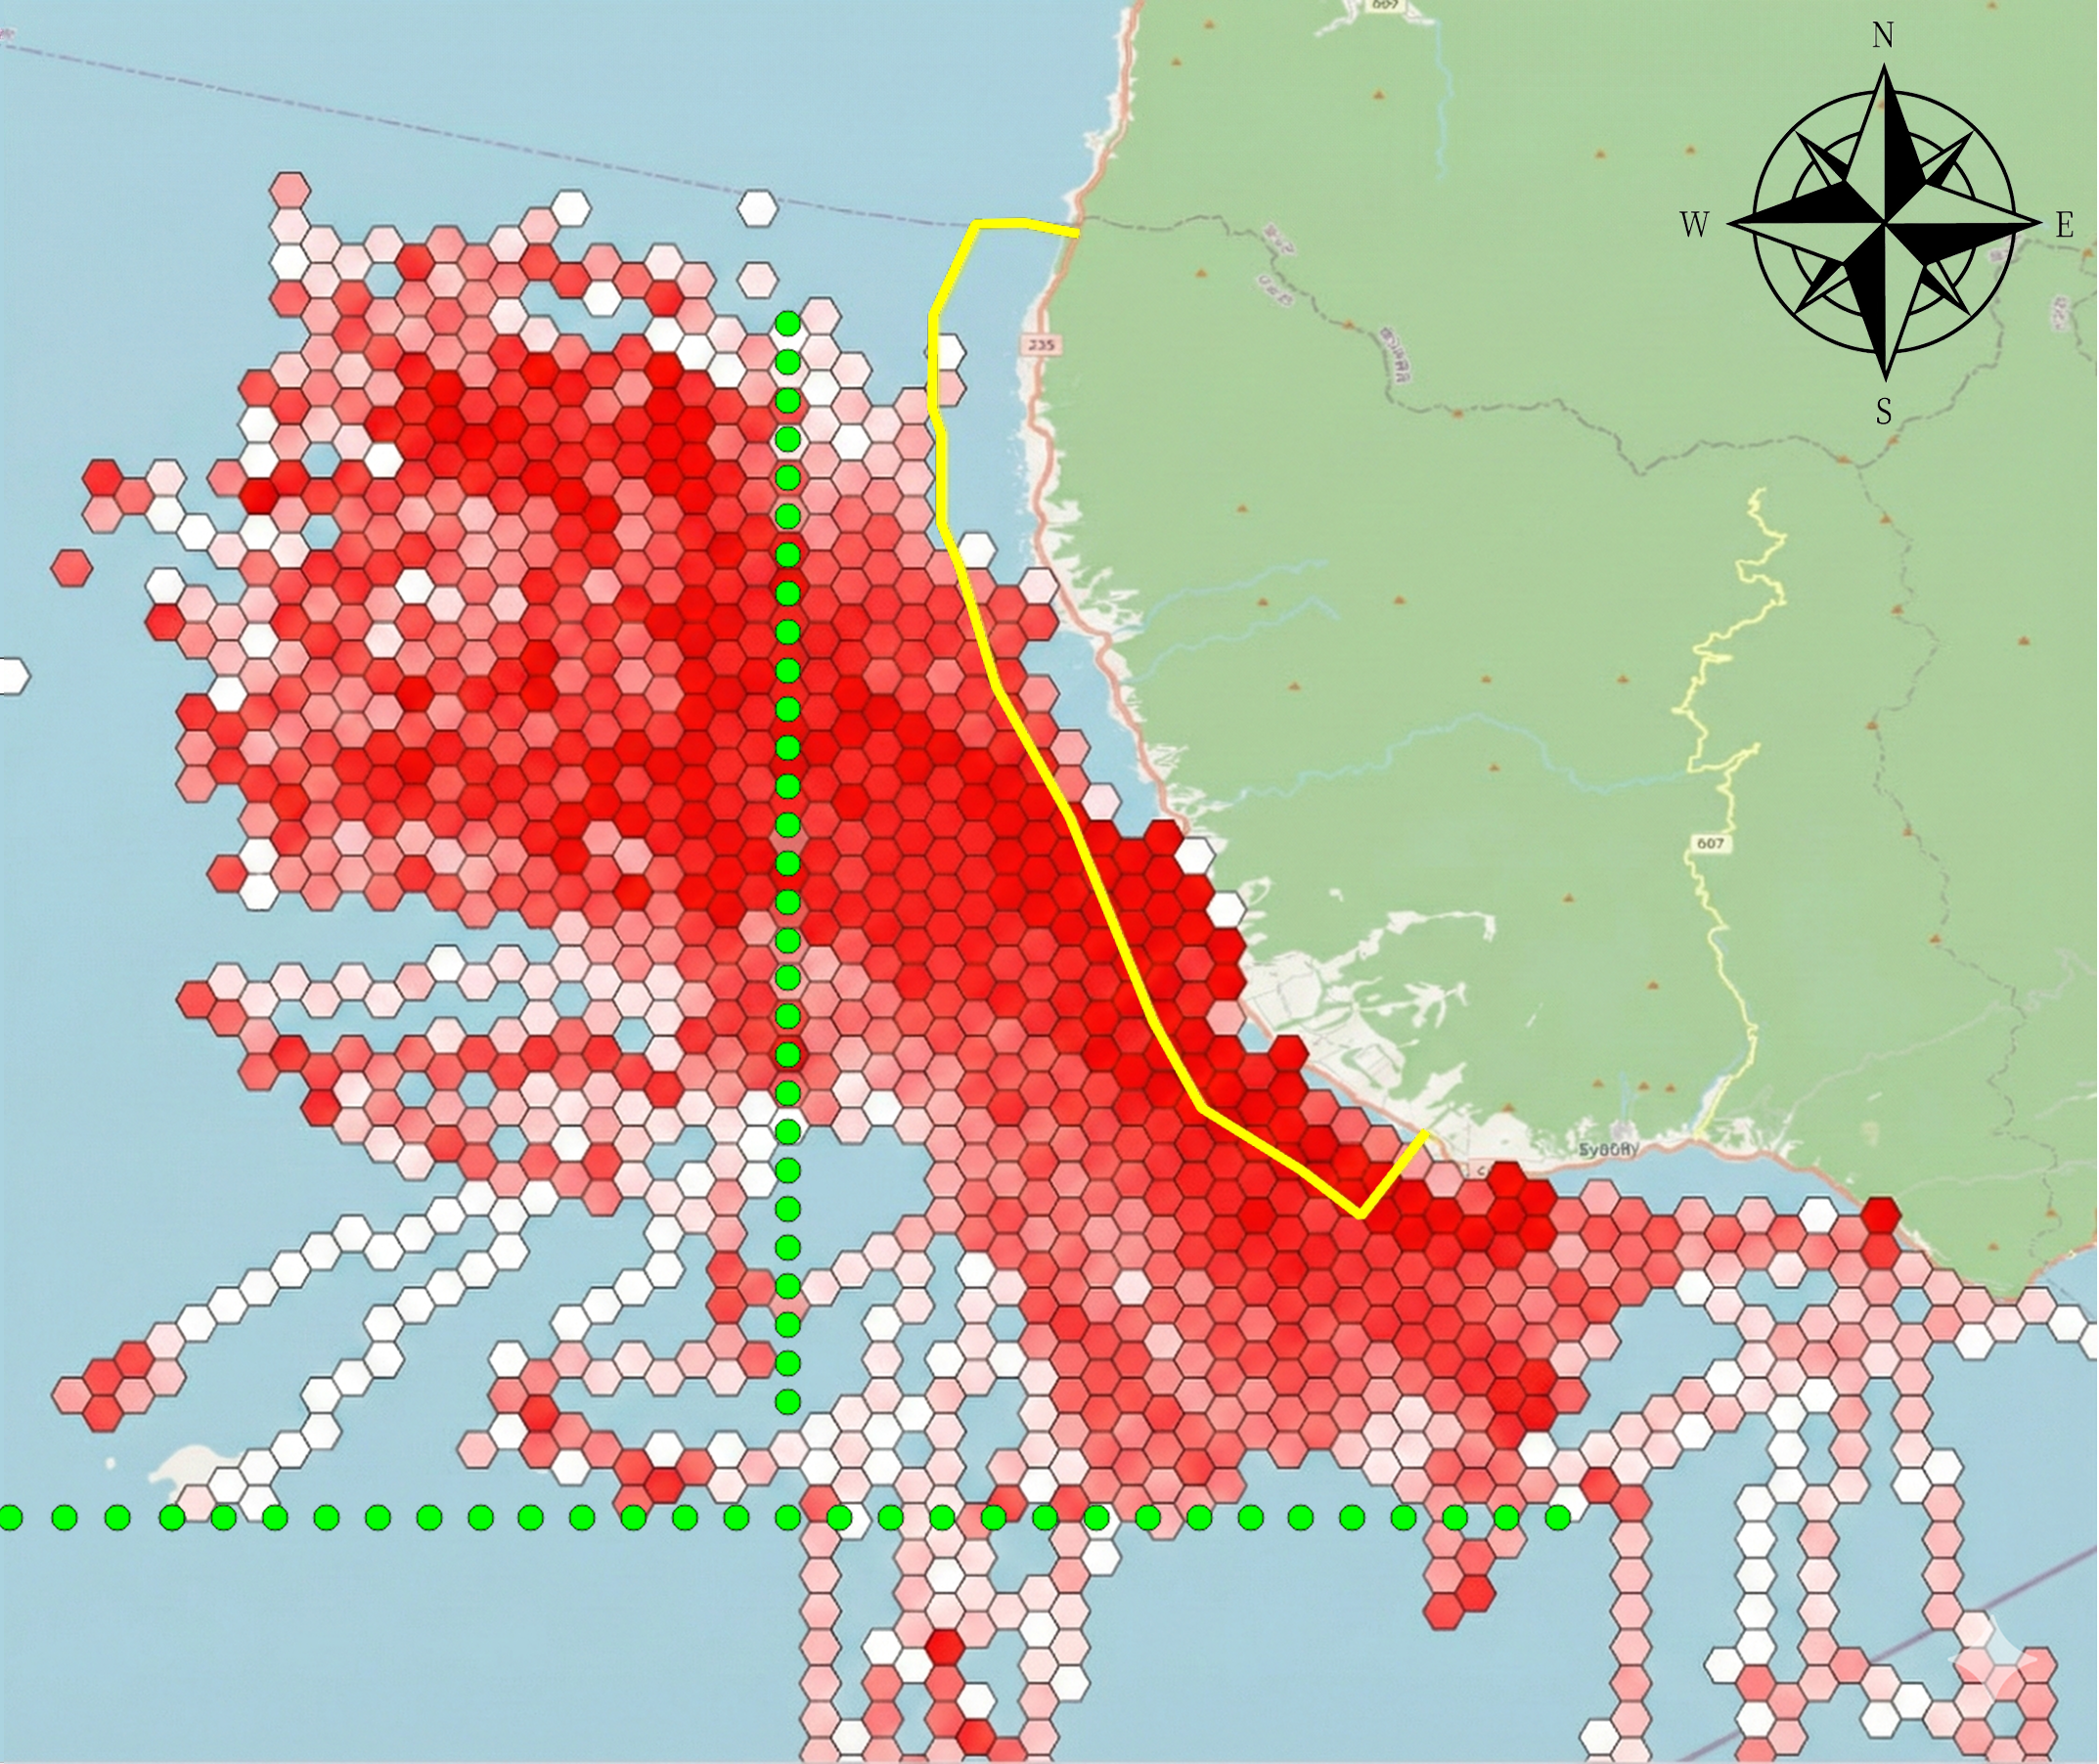
\includegraphics[width=14cm]{images/overlap.jpg}
  \caption{操業実態と洋上風車促進区域の空間的重複}
  \label{fig:overlap}
\end{figure}

図を参照すると、促進区域は【例:操業密度の高い主要漁場と直接的に重複している / 主要漁場の縁辺部に位置している】ことが確認できる。
具体的には、促進区域の【例:南西側】において、高い操業密度を示すグリッドが多数含まれており、この海域はマグロ延縄漁業において日常的に利用されている重要漁場であることが定量的に示された。
また、区域内部だけでなく、区域の【例:沖合側】にも操業実績が広がっていることから、当該区域は漁場としてだけでなく、漁場へ向かうための「移動経路」としても機能している可能性が高い。
したがって、この海域に風車が建設された場合、操業海域の喪失のみならず、迂回による移動コストの増加や、探索行動の制約といった影響が生じることが懸念される。

\section{操業効率の現状評価}
最後に、漁業への物理的・経済的負担の現状(ベースライン)を把握するため、単位努力量あたりの漁獲量(CPUE)および燃油効率の分析結果を示す。

\subsection{CPUEの推移}
1航海あたりの総移動距離(努力量)と漁獲量の関係を図\ref{fig:cpue_scatter}に、年度ごとのCPUEの分布を図\ref{fig:cpue_boxplot}に示す。

\begin{figure}[htbp]
  \centering
  % \includegraphics[width=12cm]{images/cpue_boxplot.png}
  \caption{年度ごとのCPUE(kg/km)の比較}
  \label{fig:cpue_boxplot}
\end{figure}

分析の結果、2024年の平均CPUEは【数値】kg/km であり、2025年の【数値】kg/km と比較して【増加/減少】傾向にあった。
(※ここにグラフから読み取れる傾向を書く:例「移動距離が伸びても漁獲量が増えない『空振り』の操業が増加しており、効率が低下している」など)

\subsection{燃油効率の推移}
投入された燃料(コスト)に対する生産性を示す燃油効率($E_o$)の算出結果を表\ref{tab:fuel_efficiency}に示す。

\begin{table}[htbp]
  \centering
  \caption{年度ごとの燃油効率(漁獲重量 / 給油量)}
  \label{tab:fuel_efficiency}
  \begin{tabular}{lccc}
    \hline
    年度 & 総漁獲量 (kg) & 総給油量 (L) & 燃油効率 (kg/L) \\
    \hline
    2023 & 【数値】 & 【数値】 & 【数値】 \\
    2024 & 【数値】 & 【数値】 & 【数値】 \\
    2025 & 【数値】 & 【数値】 & 【数値】 \\
    \hline
  \end{tabular}
\end{table}

表より、燃油効率は【例:年々悪化している】ことが分かる。
これは、前項で示した漁場の遠隔化(沖合シフト)や探索距離の増加に対し、漁獲量が比例して増加していないことを示唆しており、漁業経営における燃料コストの負担が増大している現状が定量的に明らかとなった。